%%%%%%%%%%%%%%%%%%%%%%%%%%%%%%%%%%%%%%%%%
% University/School Laboratory Report
% LaTeX Template
% Version 3.1 (25/3/14)
%
% This template has been downloaded from:
% http://www.LaTeXTemplates.com
%
% Original author:
% Linux and Unix Users Group at Virginia Tech Wiki 
% (https://vtluug.org/wiki/Example_LaTeX_chem_lab_report)
%
% License:
% CC BY-NC-SA 3.0 (http://creativecommons.org/licenses/by-nc-sa/3.0/)
%
%%%%%%%%%%%%%%%%%%%%%%%%%%%%%%%%%%%%%%%%%

%----------------------------------------------------------------------------------------
%	PACKAGES AND DOCUMENT CONFIGURATIONS
%----------------------------------------------------------------------------------------

\documentclass[12pt]{article}

\usepackage[hmargin=3cm, vmargin=2cm]{geometry} % set margins

\usepackage{graphicx} % Required for the inclusion of images
\usepackage{natbib} % Required to change bibliography style to APA
%\usepackage{amsmath} % Required for some math elements 
\usepackage[utf8]{inputenc} % Use UTF-8
\usepackage{float}
\usepackage{booktabs}

\setlength\parindent{0pt} % Removes all indentation from paragraphs

\graphicspath{{images/}} % Define graphics path

\renewcommand{\labelenumi}{\alph{enumi}.} % Make numbering in the enumerate environment by letter rather than number (e.g. section 6)

\renewcommand{\baselinestretch}{1.5} % set line spacing

\usepackage{times} % Uncomment to use the Times New Roman font

%----------------------------------------------------------------------------------------
%	DOCUMENT INFORMATION
%----------------------------------------------------------------------------------------

\title{Data Analysis and Knowledge Discovery \\ Exercise Work 1} % Title

\author{Tatu Seppä-Lassila} % Author name

\date{\today} % Date for the report

\begin{document}

\maketitle % Insert the title, author and date

%----------------------------------------------------------------------------------------
%	SECTIONS
%----------------------------------------------------------------------------------------
 
\section{Task 1: Histograms}

Histograms were plotted using python and matplotlib. Freedman-Diaconis rule, Sturges' rule and Square-root choice was used to calculate the number of bins in the histograms. These three histograms were plotted for all of the attributes. However, only plots for alcohol are shown in this documents to demonstrate the results. 

% Histogram, Freedman Diaconis
\begin{figure}[H]
    \centering
    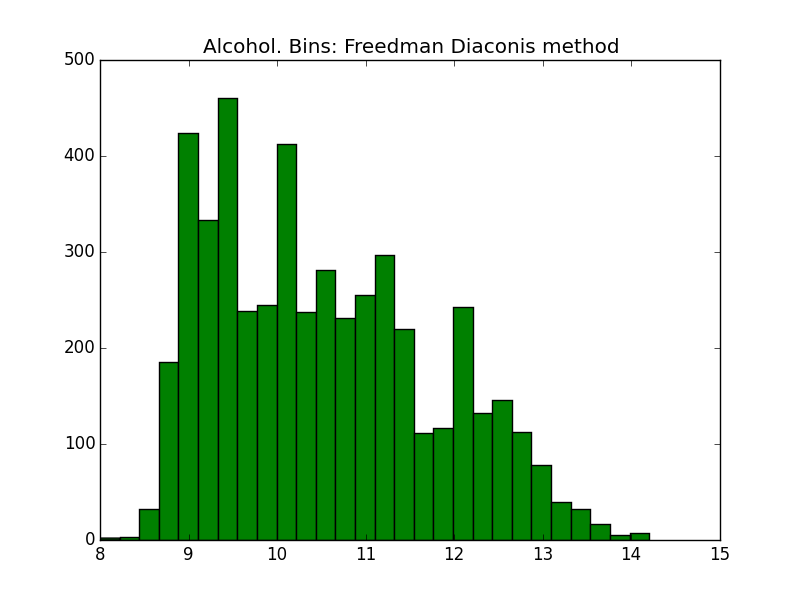
\includegraphics[width=0.8\textwidth]{alcohol_fdr}
    \caption{Histogram of alcohol attribute. Number of bins selected with Freedman-Diaconis rule.}
    \label{fig:histogram_fdr}
\end{figure}
% End of picture

% Histogram, Freedman Diaconis
\begin{figure}[H]
    \centering
    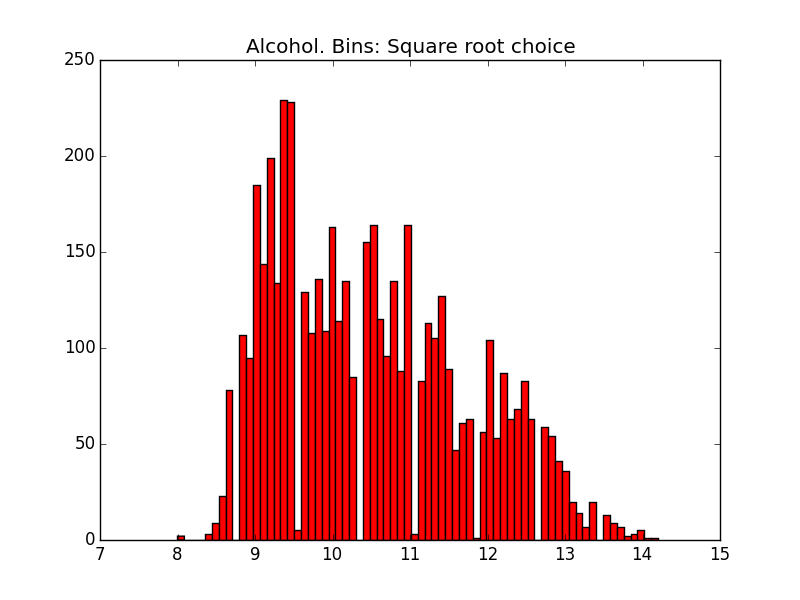
\includegraphics[width=0.85\textwidth]{alcohol_src}
    \caption{Histogram of alcohol attribute. Number of bins selected with Square-root choice.}
    \label{fig:histogram_src}
\end{figure}
% End of picture

% Histogram, Sturges' rule
\begin{figure}[H]
    \centering
    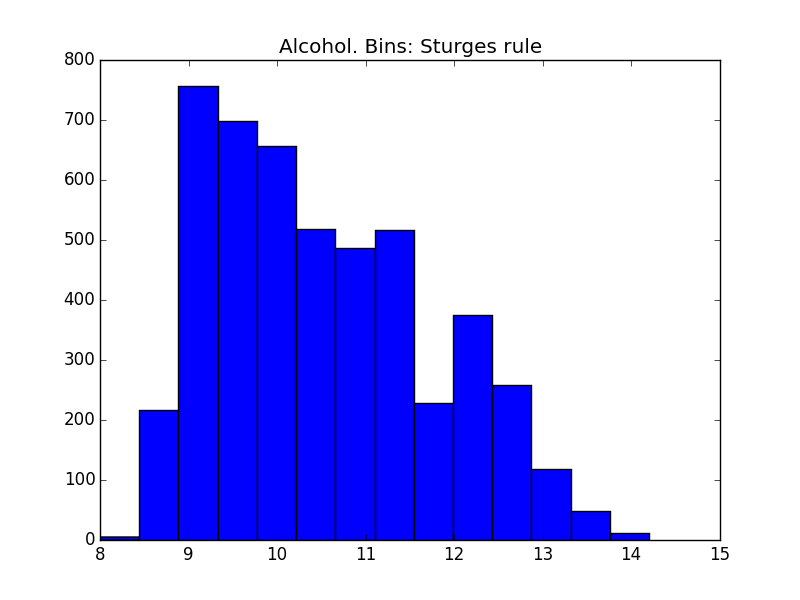
\includegraphics[width=0.85\textwidth]{alcohol_sturge}
    \caption{Histogram of alcohol attribute. Number of bins selected with Sturges' rule.}
    \label{fig:histogram_sturge}
\end{figure}
% End of picture

Figures \ref{fig:histogram_fdr}, \ref{fig:histogram_src}, \ref{fig:histogram_sturge} show the plotted histograms for alcohol attribute. Square-root choice produced 70 bins with this dataset. Respectively, Freedman-Diaconis rule produced 28 bins and Sturges' 14 bins. Histograms with lower number of bins show that majority of samples have alcohol around 10. Figure \ref{fig:histogram_src} shows that higher number of bins reveal that some tenths have very low number of samples, even though the next tenth has 50 or more samples.%

\section{Task 2: Scatter Plots and Parallel Coordinates Representation}

\subsection{Scatter plots}

Scatter plots were produced using matplotlib's scatter function. Attributes were plotted against each other, but only three were added to this document.

% Scatter plot, density and sulphates
\begin{figure}[H]
    \centering
    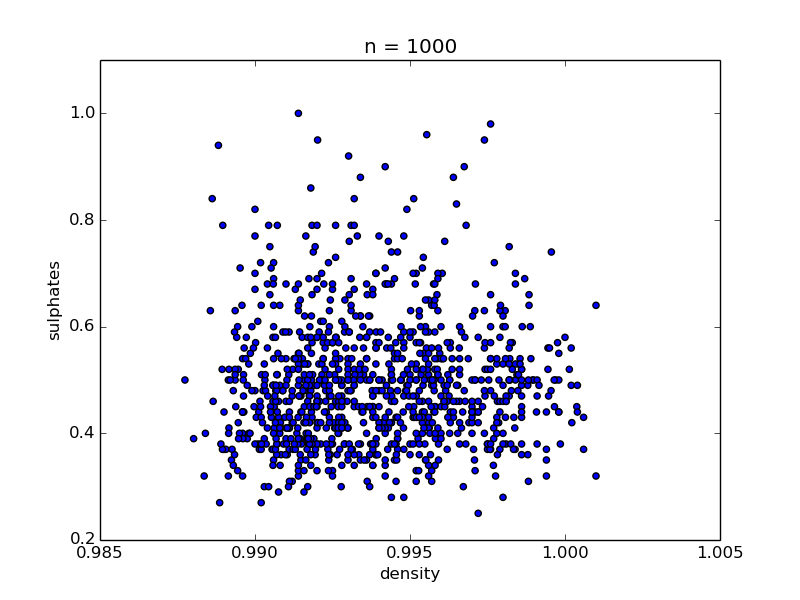
\includegraphics[width=0.9\textwidth]{scatter_plot_density_sulphates}
    \caption{Scatter plot of density and sulphates}
    \label{fig:scatter_dens_sulph}
\end{figure}
% End of picture

% Scatter plot, ph and alcohol
\begin{figure}[H]
    \centering
    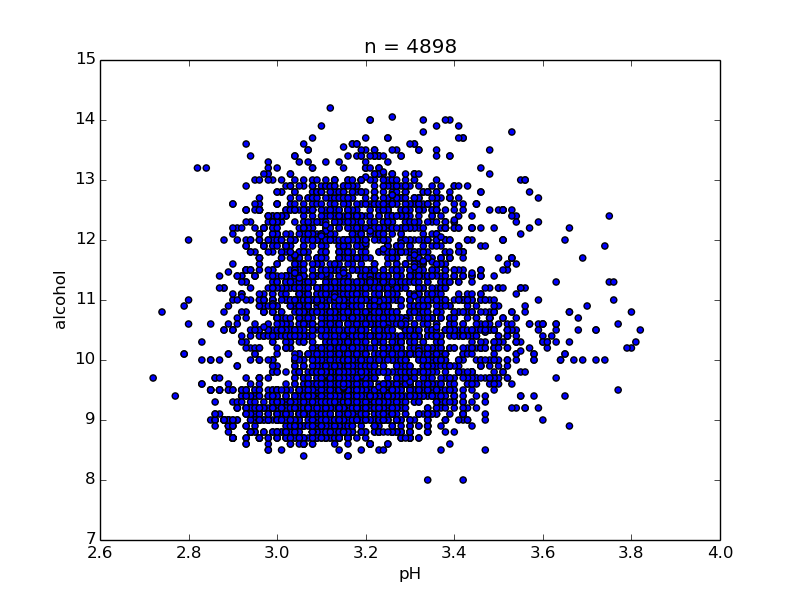
\includegraphics[width=0.85\textwidth]{scatter_plot_pH_alcohol}
    \caption{Scatter plot of pH and alcohol}
    \label{fig:scatter_ph_alc}
\end{figure}
% End of picture

% Scatter plot, residual sugar and free sulfur dioxide
\begin{figure}[H]
    \centering
    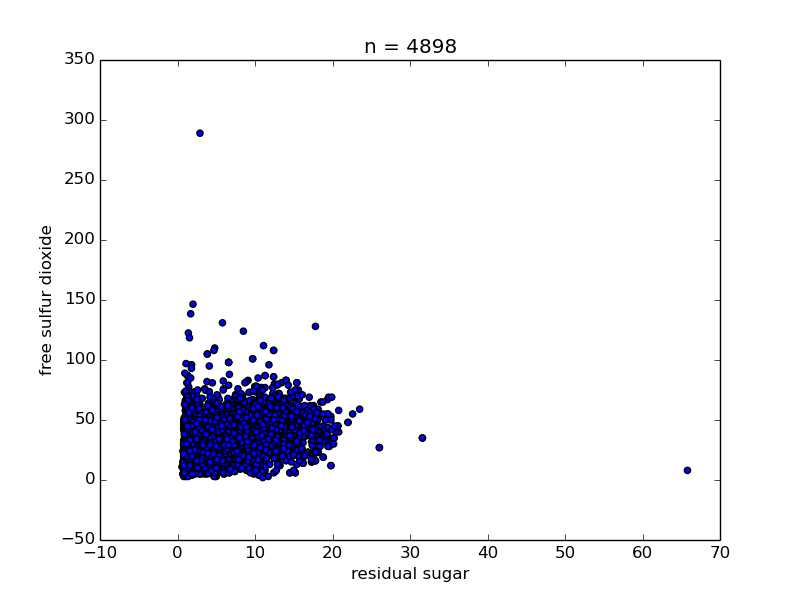
\includegraphics[width=0.85\textwidth]{scatter_plot_residual_sugar_free_sulfur_dioxide}
    \caption{Scatter plot of residual sugar and free sulfur dioxide}
    \label{fig:scatter_rs_fsd}
\end{figure}
% End of picture

Figure \ref{fig:scatter_dens_sulph} shows how samples are omitted to make the density variations more visible. Figure \ref{fig:scatter_ph_alc} shows how samples have quite evenly scattered pH values relative to alcohol. Figure \ref{fig:scatter_rs_fsd} shows some outliers.

\subsection{Parallel coordinates representation}

Parallel coordinates representation were plotted with pandas' parallel\_coordinates method. The samples are plotted against quality attribute.

% Parallel, raw
\begin{figure}[H]
    \centering
    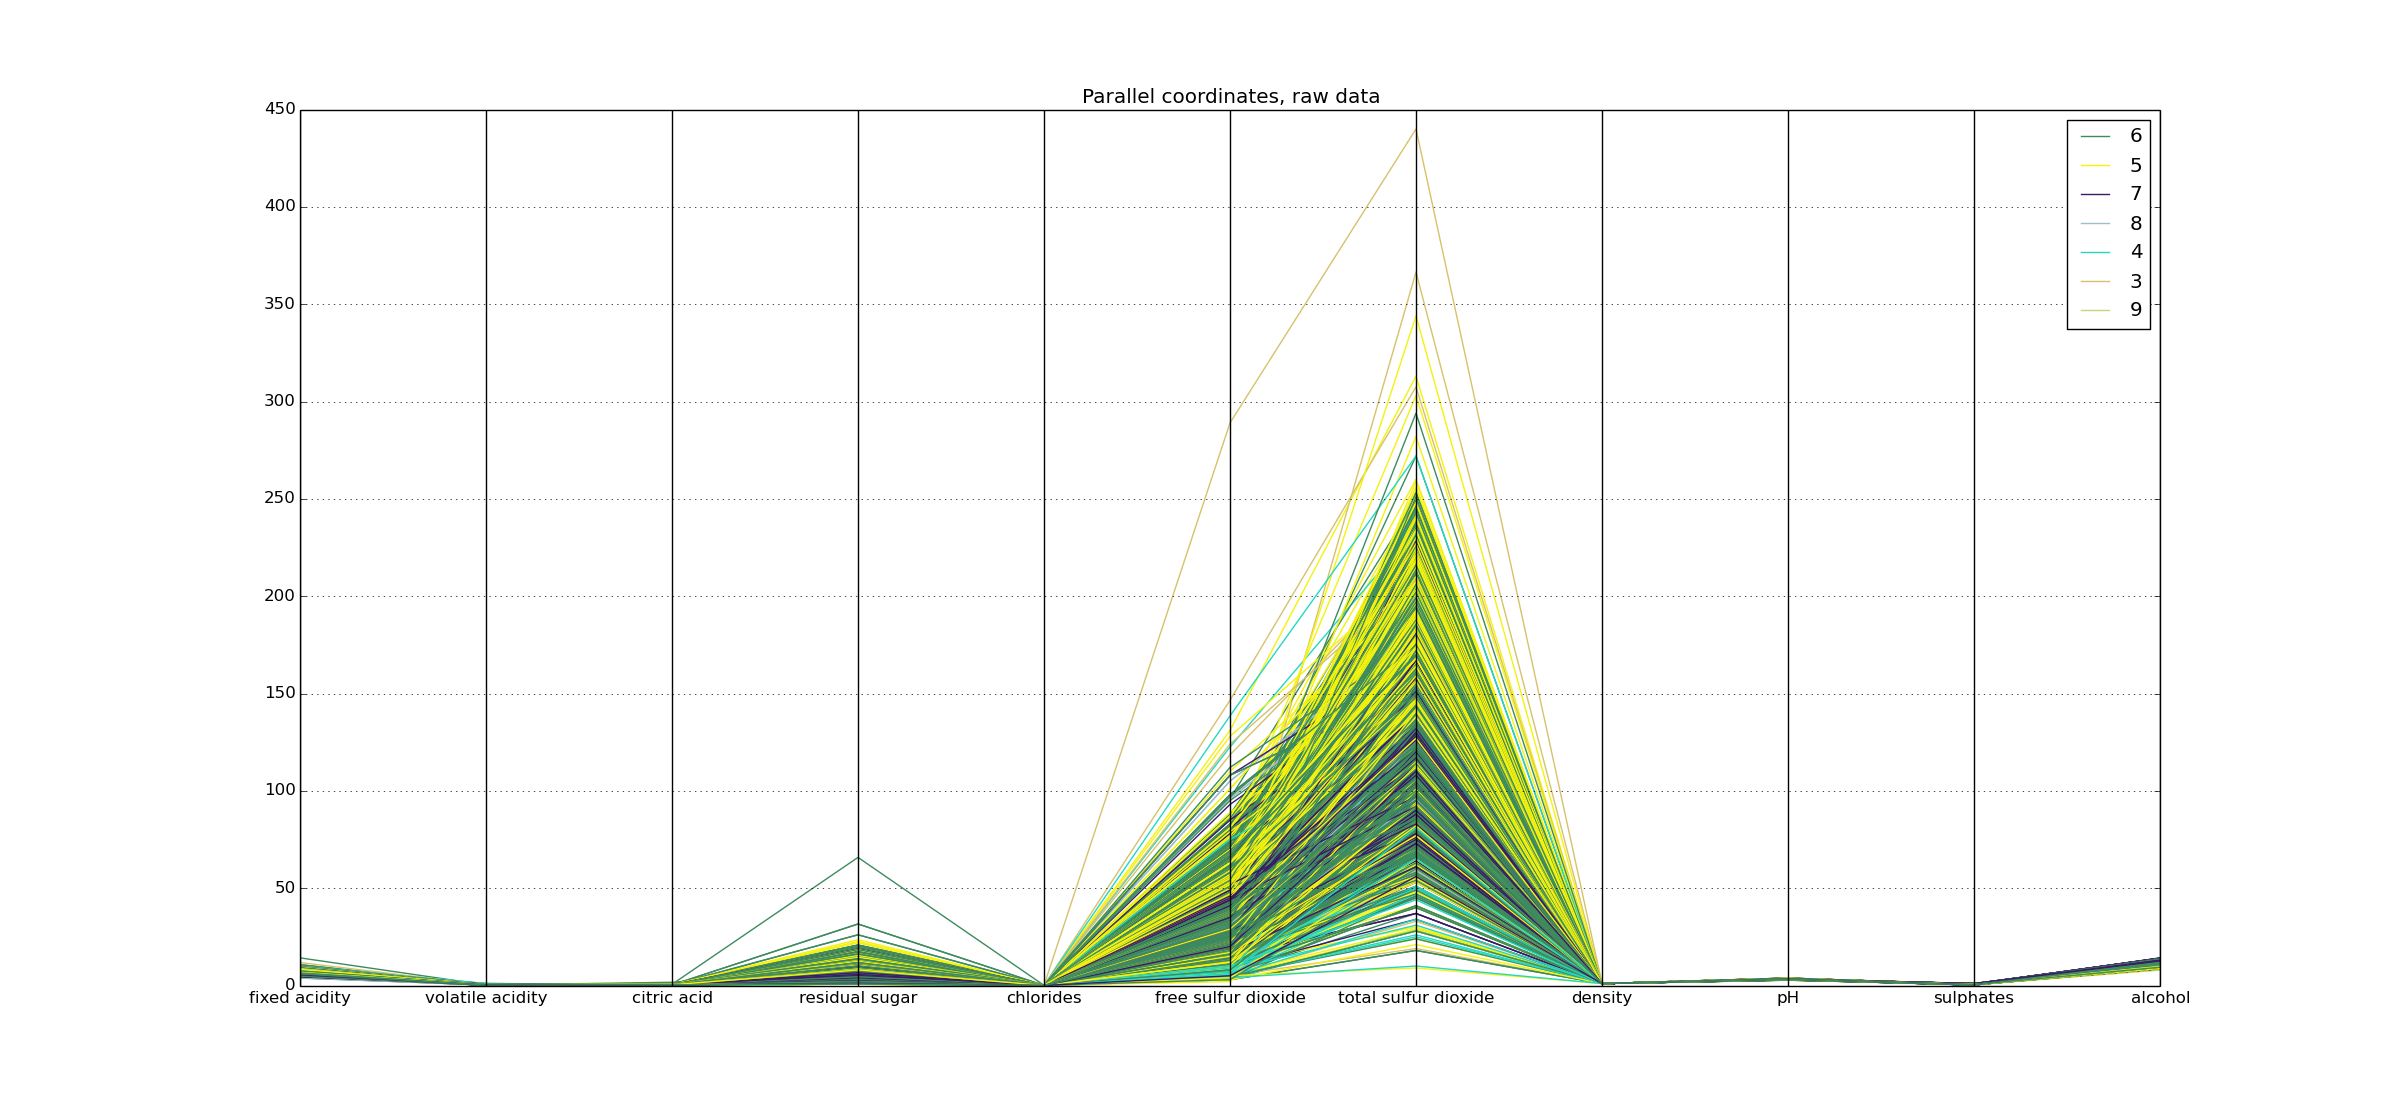
\includegraphics[width=1\textwidth]{parallel_raw}
    \caption{Parallel coordinates representation with raw data values}
    \label{fig:parallel_raw}
\end{figure}
% End of picture

% Parallel, scaled
\begin{figure}[H]
    \centering
    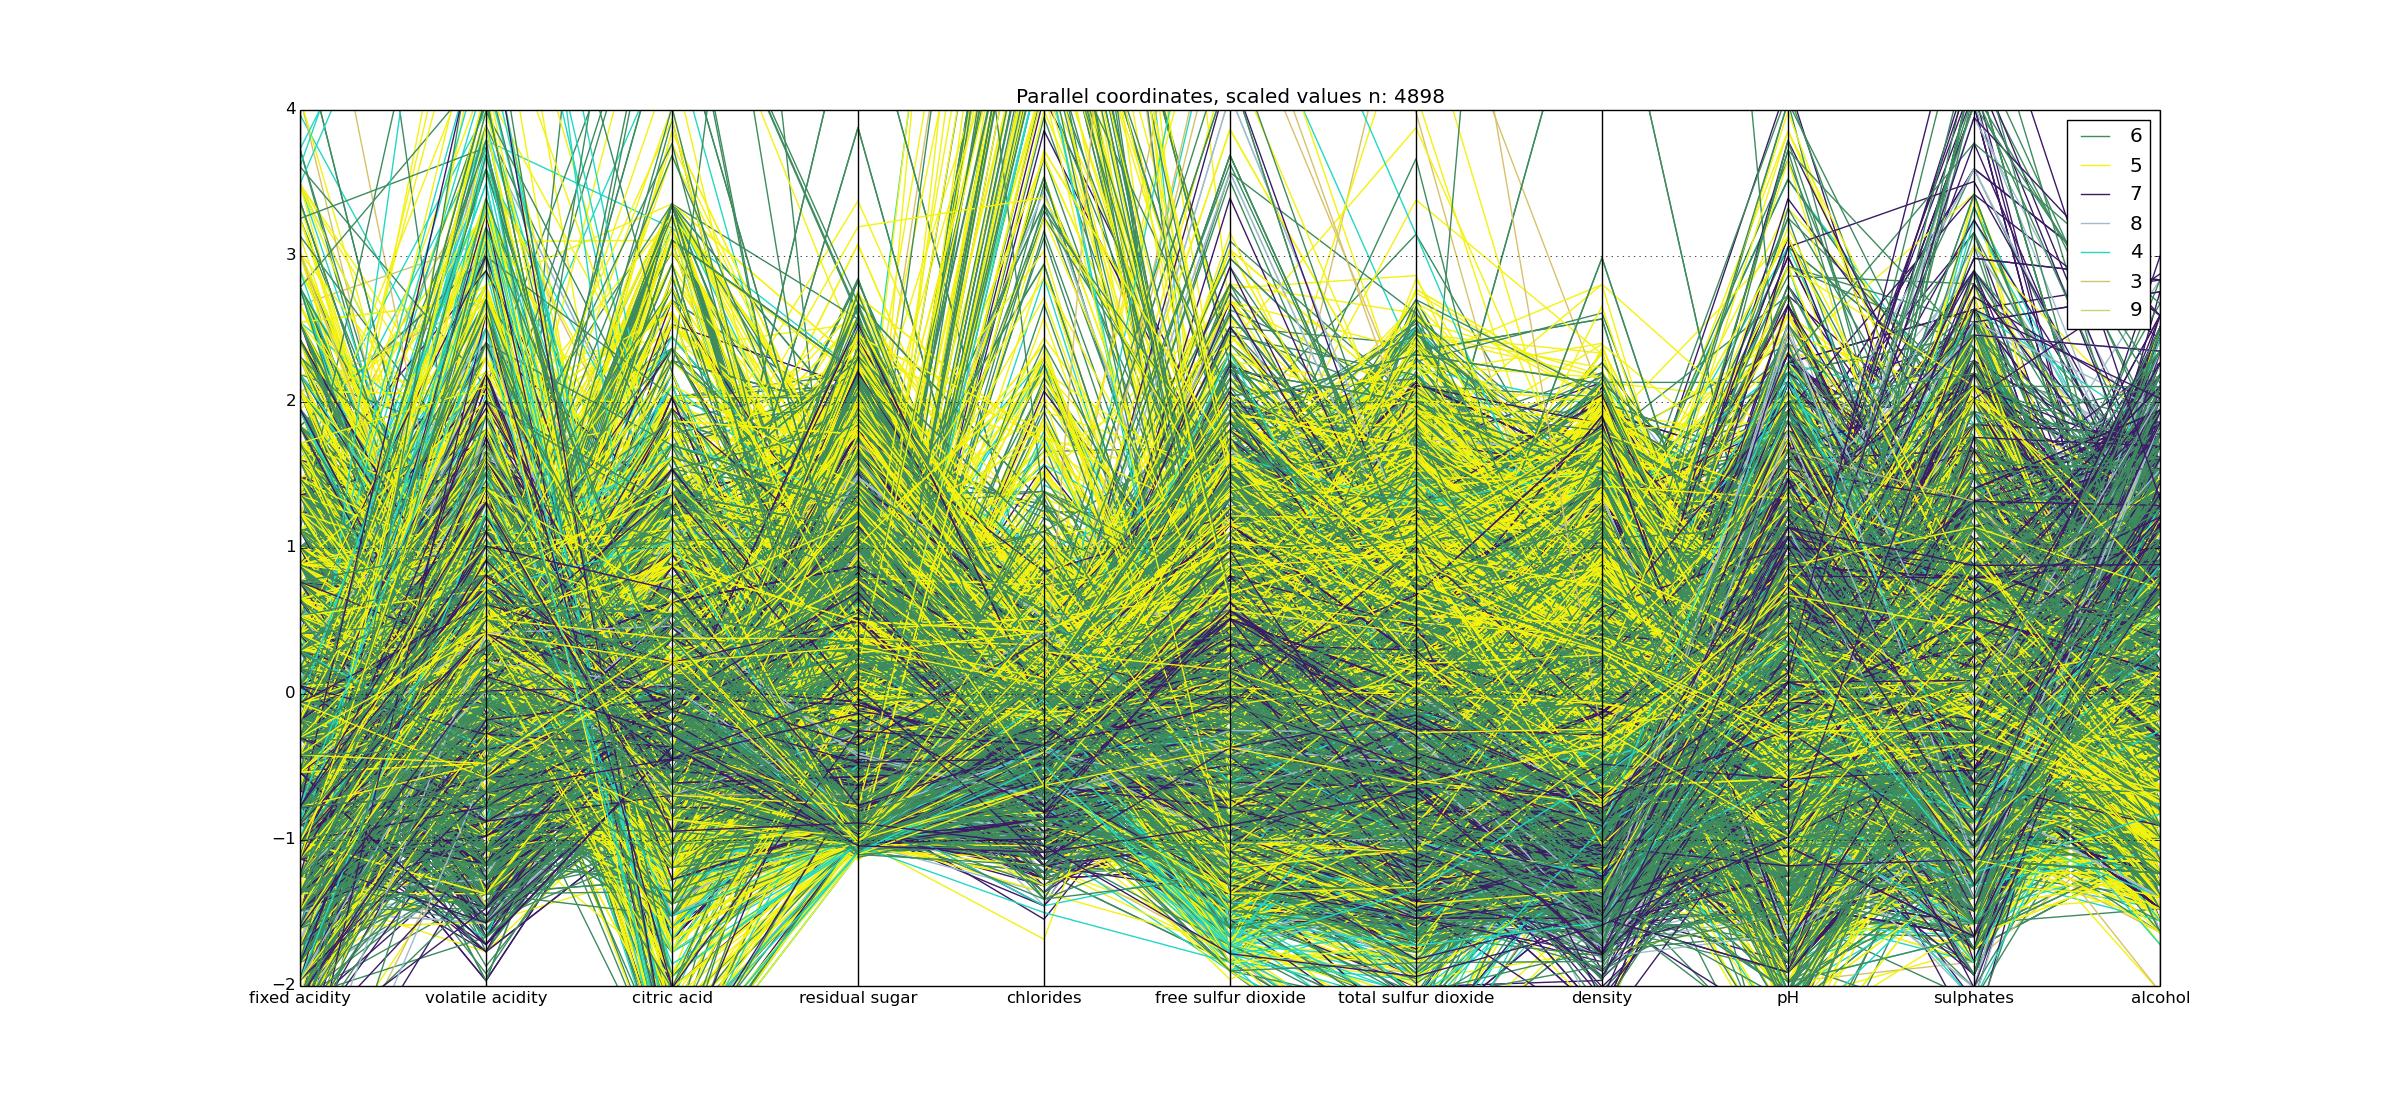
\includegraphics[width=1\textwidth]{parallel_scaled}
    \caption{Parallel coordinates representation with scaled data values}
    \label{fig:parallel_scaled}
\end{figure}
% End of picture

% Parallel, scaled, subsample
\begin{figure}[H]
    \centering
    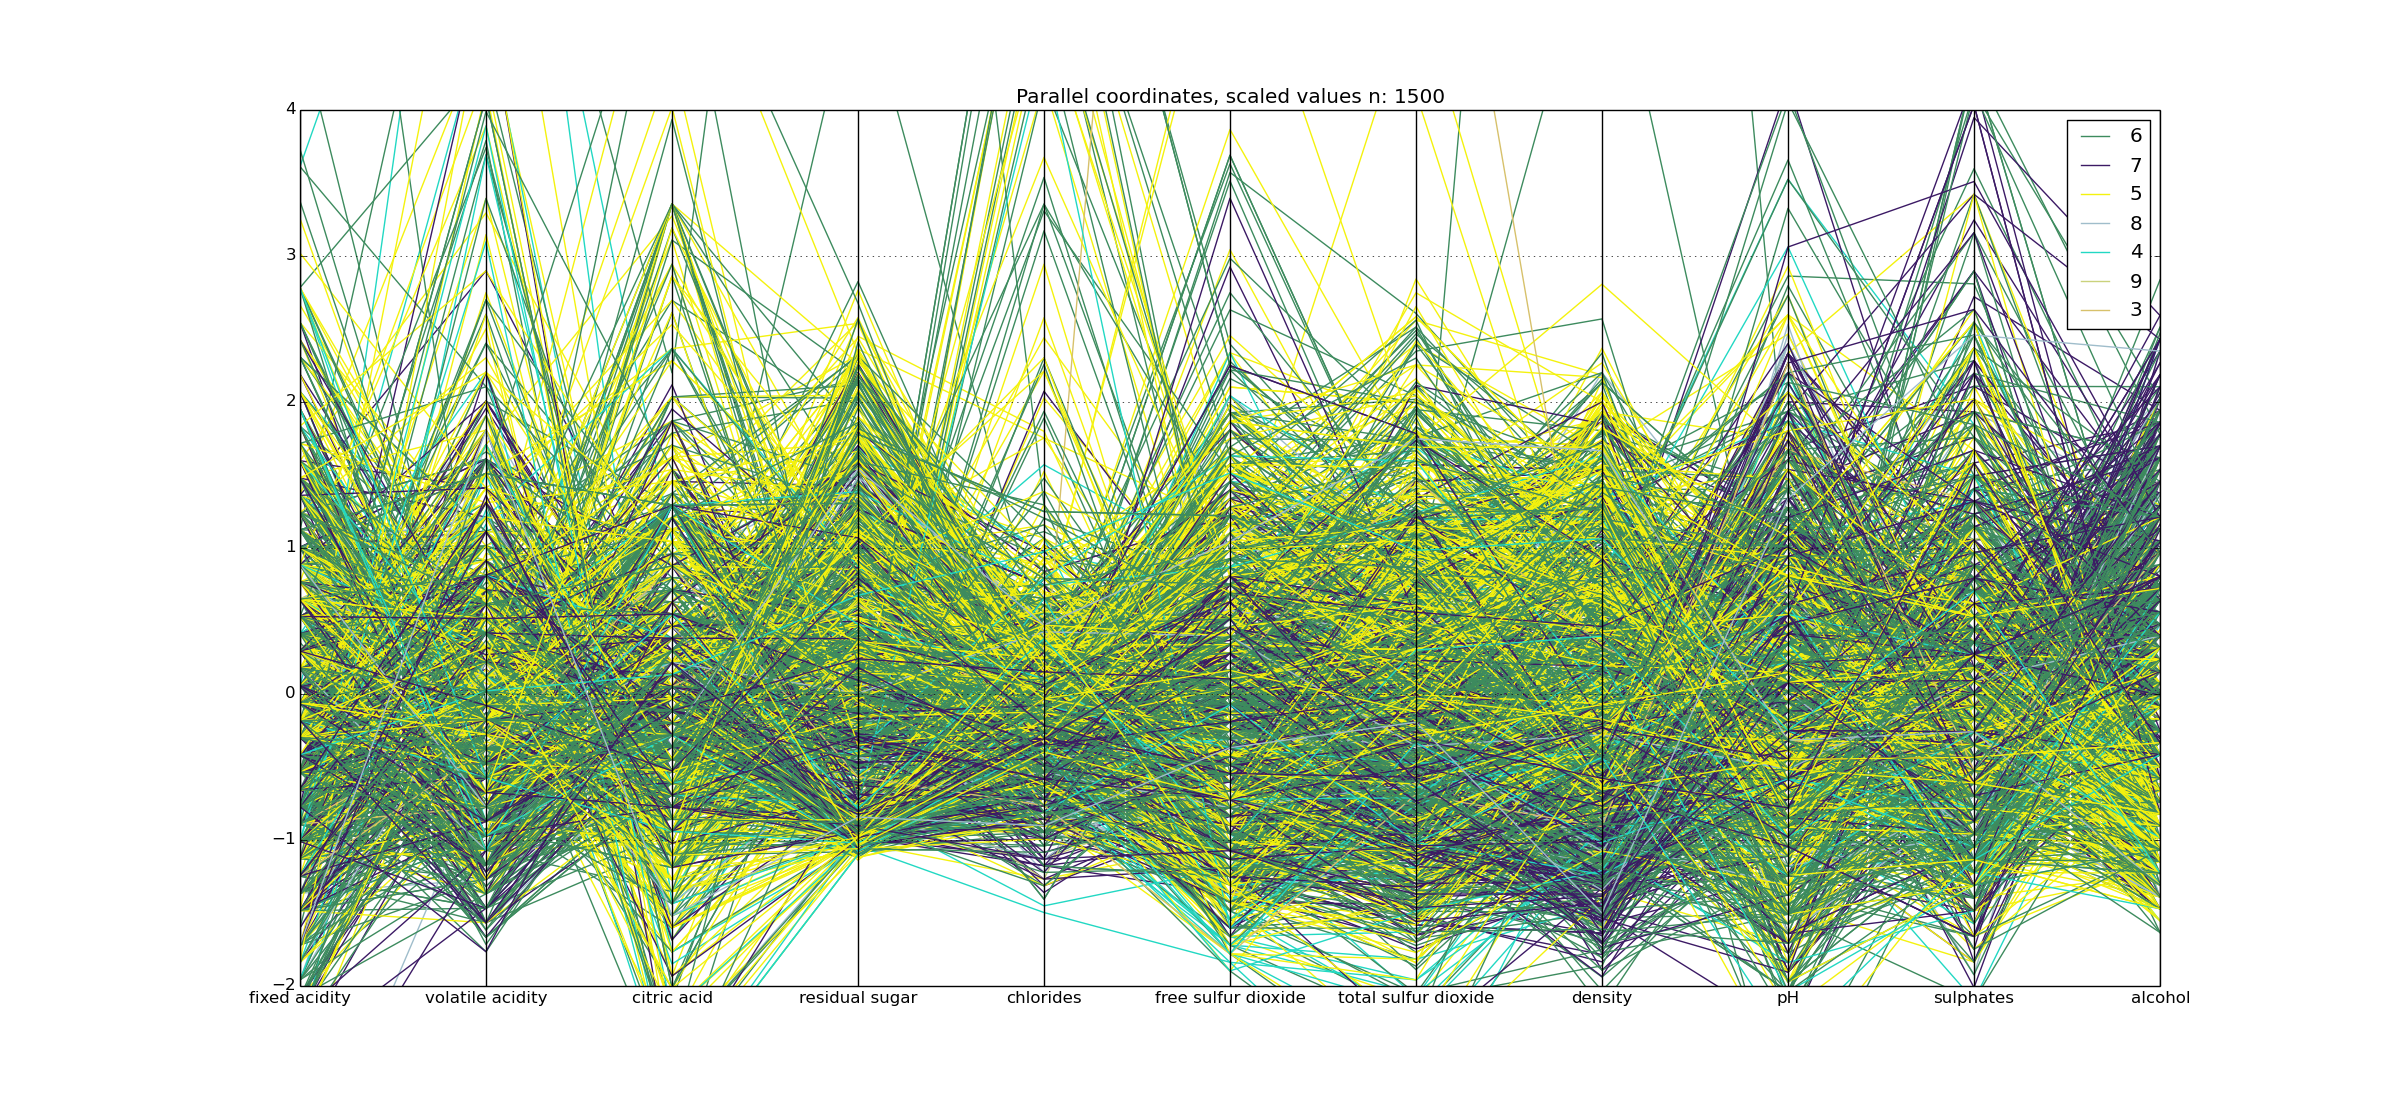
\includegraphics[width=1\textwidth]{parallel_scaled_subsample}
    \caption{Parallel coordinates representation with scaled data values. Number of samples is limited to 1500}
    \label{fig:parallel_scaled_subsample}
\end{figure}
% End of picture

The method does not allow attributes to be scaled independently. Figure \ref{fig:parallel_raw} shows the plotted figure and it can be seen that this figure is not very useful for data understanding. That is why the data values were scaled, which can be seen in Figure \ref{fig:parallel_scaled}. Figure \ref{fig:parallel_scaled_subsample} shows the same image with number of samples limited to 1500 to provide a bit clearer picture.

\section{Task 3: Principal Component Analysis}

PCA component analysis was done using numpy's cov method to calculate covariance matrix and linalg.eig to calculate eigen vectors and eigen values. The figure was done using matplotlib's plot method.

% PCA, raw
\begin{figure}[H]
    \centering
    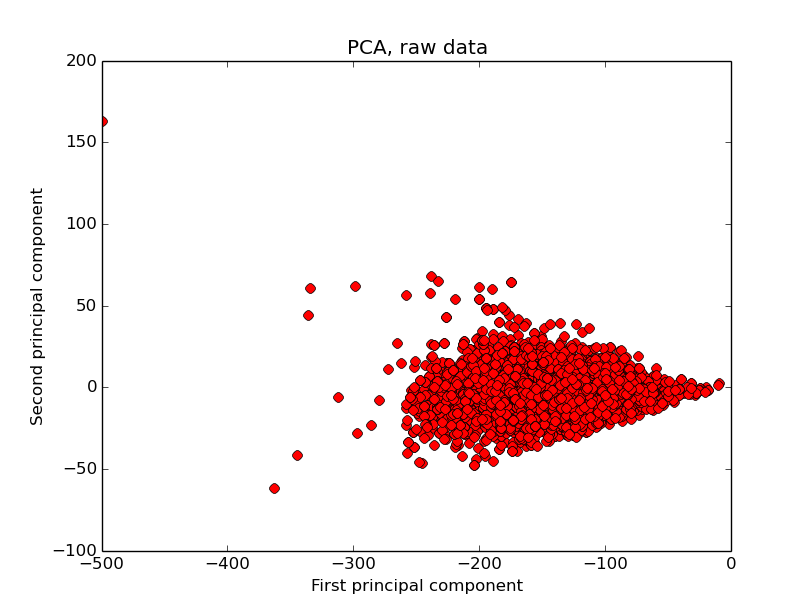
\includegraphics[width=0.8\textwidth]{pca_raw}
    \caption{PCA with raw data}
    \label{fig:pca_raw}
\end{figure}
% End of picture

% PCA, normalized
\begin{figure}[H]
    \centering
    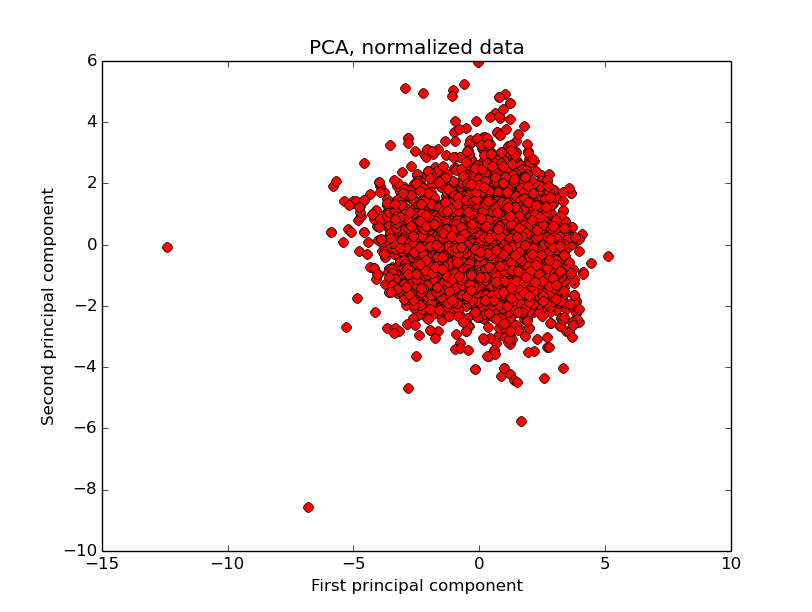
\includegraphics[width=0.8\textwidth]{pca_normalized}
    \caption{PCA with z-score normalized data}
    \label{fig:pca_normalized}
\end{figure}
% End of picture

Figure \ref{fig:pca_raw} shows scatter plot of the first two principal components computed with raw data. Figure \ref{fig:pca_normalized} shows the same scatter plot with normalized data. With normalization, the scatter plot shows more rounded figure compared to raw data which has kind of triangle shape.

\section{Task 4: 2D Multidimensional Scaling}

2D MDS was calculated with MDS function from scikit-learn. The figure was done using matplotlib's plot method.

% 2D MDS
\begin{figure}[H]
    \centering
    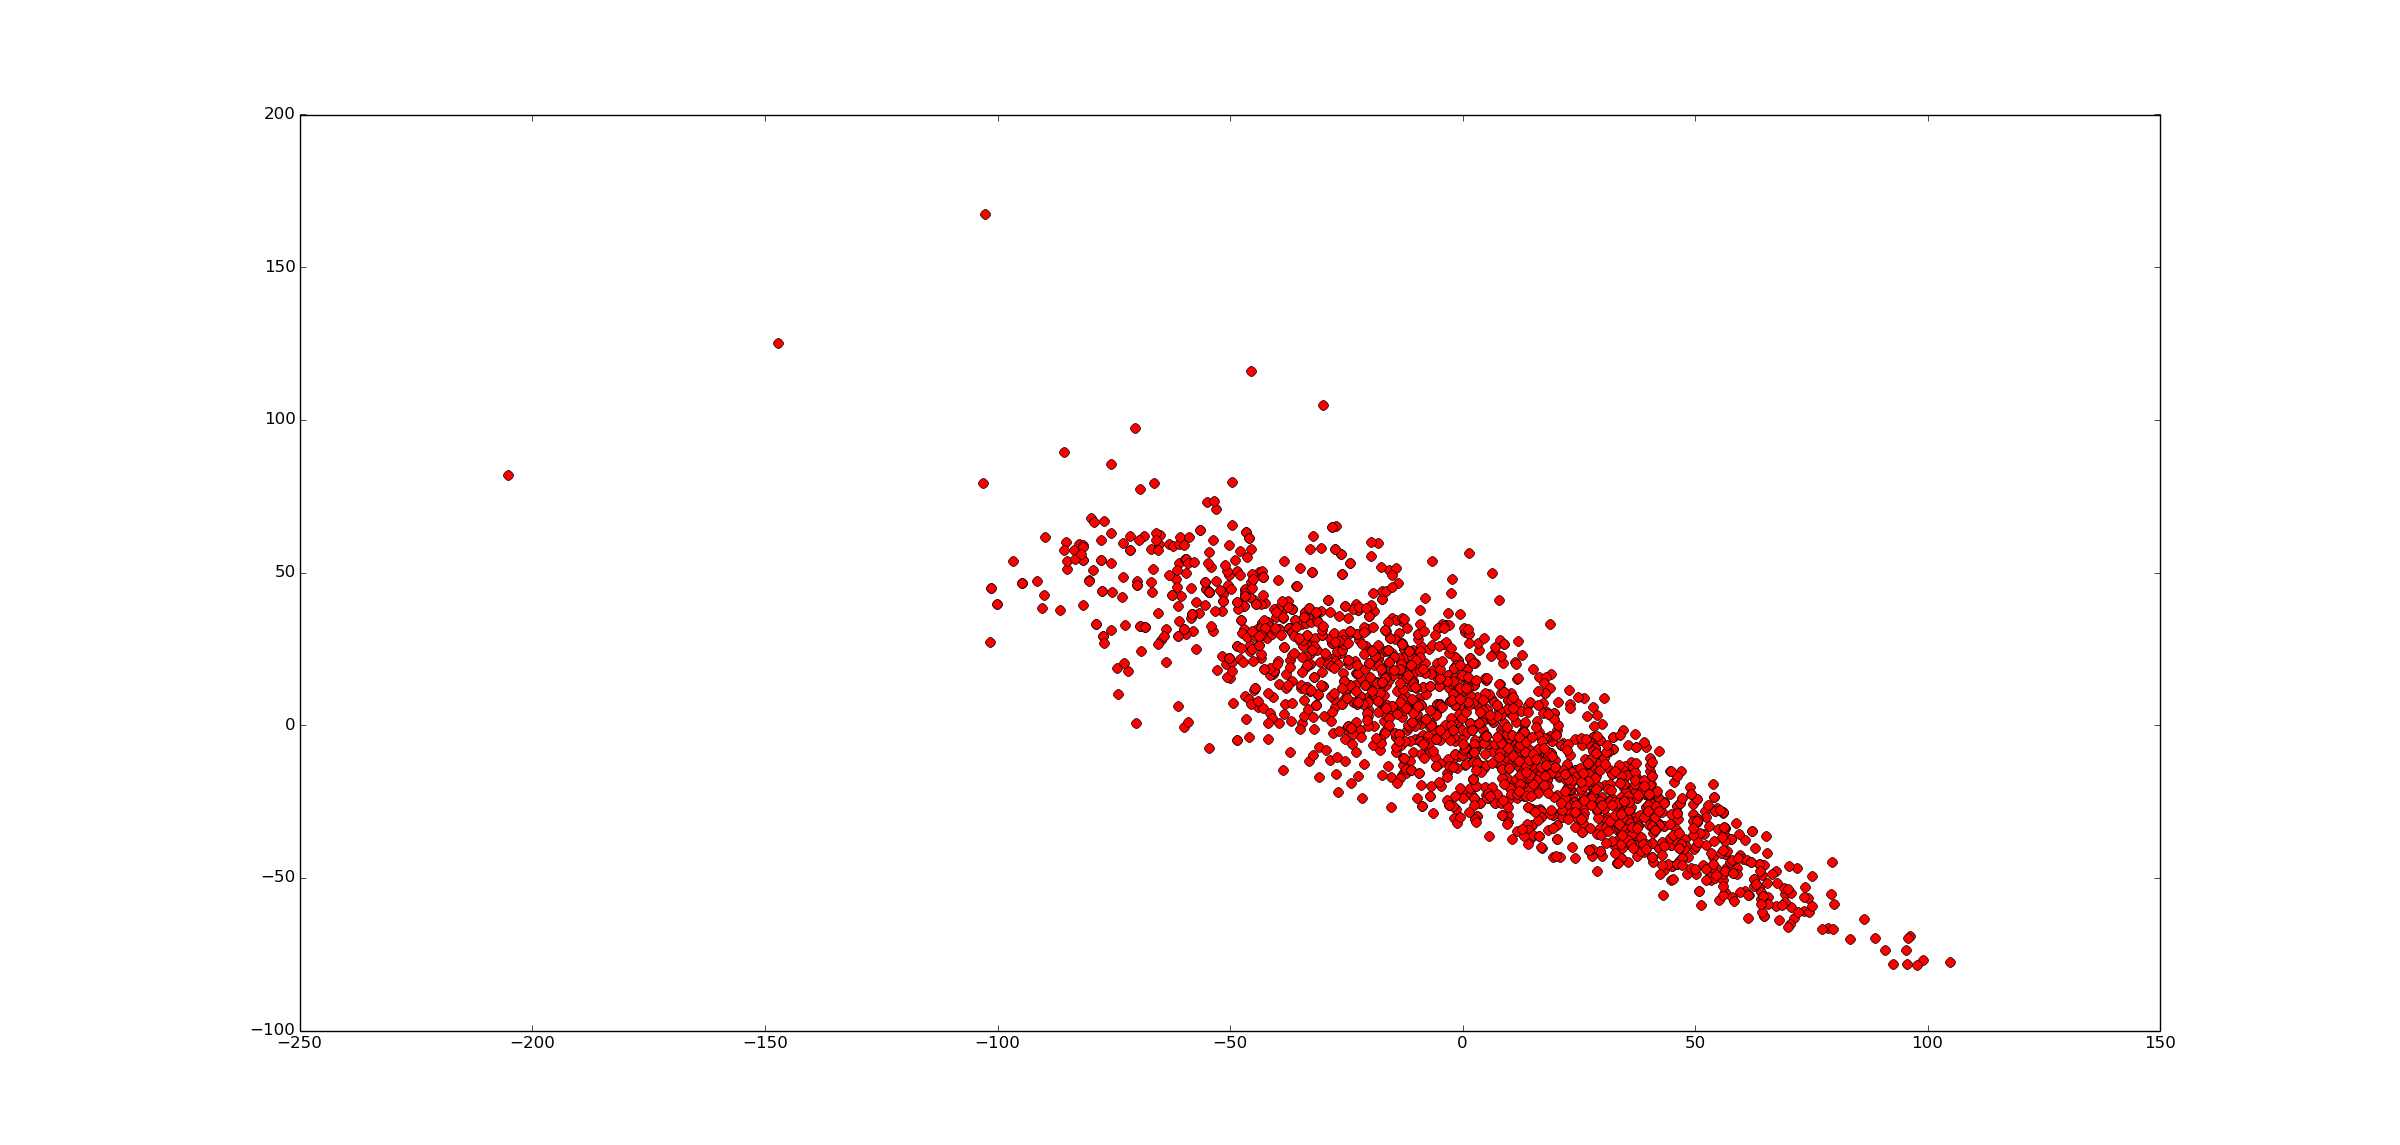
\includegraphics[width=0.8\textwidth]{2d_mds}
    \caption{2D MDS}
    \label{fig:mds}
\end{figure}
% End of picture

Figure \ref{fig:mds} shows 2D MDS scatter plot. The figure has some resemblence to PCA scatter plot with raw data as data points are more scattered on the direction of x-axis. 2D MDS scatter plot shows negative correlation between the dimensions, whereas this is not visible in PCA scatter plots between the princial components.

\section{Task 5: Pearson and Kendall's Tau Correlation Tables}

Correlation tables were calculated with Pandas' "corr" method.

\subsection{Pearson Correlation Table}

\resizebox{\linewidth}{!}{%

\begin{tabular}{lrrrrrrrrrrrr}
\toprule
{} &  fixed acidity &  volatile acidity &  citric acid &  residual sugar &  chlorides &  free sulfur dioxide &  total sulfur dioxide &   density &        pH &  sulphates &   alcohol &   quality \\
\midrule
fixed acidity        &       1.000000 &         -0.022697 &     0.289181 &        0.089021 &   0.023086 &            -0.049396 &              0.091070 &  0.265331 & -0.425858 &  -0.017143 & -0.120881 & -0.113663 \\
volatile acidity     &      -0.022697 &          1.000000 &    -0.149472 &        0.064286 &   0.070512 &            -0.097012 &              0.089261 &  0.027114 & -0.031915 &  -0.035728 &  0.067718 & -0.194723 \\
citric acid          &       0.289181 &         -0.149472 &     1.000000 &        0.094212 &   0.114364 &             0.094077 &              0.121131 &  0.149503 & -0.163748 &   0.062331 & -0.075729 & -0.009209 \\
residual sugar       &       0.089021 &          0.064286 &     0.094212 &        1.000000 &   0.088685 &             0.299098 &              0.401439 &  0.838966 & -0.194133 &  -0.026664 & -0.450631 & -0.097577 \\
chlorides            &       0.023086 &          0.070512 &     0.114364 &        0.088685 &   1.000000 &             0.101392 &              0.198910 &  0.257211 & -0.090439 &   0.016763 & -0.360189 & -0.209934 \\
free sulfur dioxide  &      -0.049396 &         -0.097012 &     0.094077 &        0.299098 &   0.101392 &             1.000000 &              0.615501 &  0.294210 & -0.000618 &   0.059217 & -0.250104 &  0.008158 \\
total sulfur dioxide &       0.091070 &          0.089261 &     0.121131 &        0.401439 &   0.198910 &             0.615501 &              1.000000 &  0.529881 &  0.002321 &   0.134562 & -0.448892 & -0.174737 \\
density              &       0.265331 &          0.027114 &     0.149503 &        0.838966 &   0.257211 &             0.294210 &              0.529881 &  1.000000 & -0.093591 &   0.074493 & -0.780138 & -0.307123 \\
pH                   &      -0.425858 &         -0.031915 &    -0.163748 &       -0.194133 &  -0.090439 &            -0.000618 &              0.002321 & -0.093591 &  1.000000 &   0.155951 &  0.121432 &  0.099427 \\
sulphates            &      -0.017143 &         -0.035728 &     0.062331 &       -0.026664 &   0.016763 &             0.059217 &              0.134562 &  0.074493 &  0.155951 &   1.000000 & -0.017433 &  0.053678 \\
alcohol              &      -0.120881 &          0.067718 &    -0.075729 &       -0.450631 &  -0.360189 &            -0.250104 &             -0.448892 & -0.780138 &  0.121432 &  -0.017433 &  1.000000 &  0.435575 \\
quality              &      -0.113663 &         -0.194723 &    -0.009209 &       -0.097577 &  -0.209934 &             0.008158 &             -0.174737 & -0.307123 &  0.099427 &   0.053678 &  0.435575 &  1.000000 \\
\bottomrule
\end{tabular}


}

\subsection{Kendall's Tau Correlation Table}

\resizebox{\linewidth}{!}{%

\begin{tabular}{lrrrrrrrrrrrr}
\toprule
{} &  fixed acidity &  volatile acidity &  citric acid &  residual sugar &  chlorides &  free sulfur dioxide &  total sulfur dioxide &   density &        pH &  sulphates &   alcohol &   quality \\
\midrule
fixed acidity        &       1.000000 &         -0.029565 &     0.208569 &        0.074946 &   0.065361 &            -0.016940 &              0.077272 &  0.185510 & -0.294796 &  -0.008724 & -0.073241 & -0.065474 \\
volatile acidity     &      -0.029565 &          1.000000 &    -0.104012 &        0.072757 &  -0.003523 &            -0.054751 &              0.081319 &  0.006600 & -0.030385 &  -0.011580 &  0.023495 & -0.154787 \\
citric acid          &       0.208569 &         -0.104012 &     1.000000 &        0.015329 &   0.022292 &             0.060809 &              0.062188 &  0.061542 & -0.101307 &   0.054489 & -0.019981 &  0.014557 \\
residual sugar       &       0.074946 &          0.072757 &     0.015329 &        1.000000 &   0.155274 &             0.236748 &              0.293319 &  0.588989 & -0.125553 &  -0.002545 & -0.305601 & -0.063087 \\
chlorides            &       0.065361 &         -0.003523 &     0.022292 &        0.155274 &   1.000000 &             0.113851 &              0.257075 &  0.349119 & -0.037891 &   0.062555 & -0.404039 & -0.244856 \\
free sulfur dioxide  &      -0.016940 &         -0.054751 &     0.060809 &        0.236748 &   0.113851 &             1.000000 &              0.444696 &  0.217295 & -0.005229 &   0.035621 & -0.182539 &  0.017164 \\
total sulfur dioxide &       0.077272 &          0.081319 &     0.062188 &        0.293319 &   0.257075 &             0.444696 &              1.000000 &  0.388378 & -0.008421 &   0.108697 & -0.325826 & -0.151230 \\
density              &       0.185510 &          0.006600 &     0.061542 &        0.588989 &   0.349119 &             0.217295 &              0.388378 &  1.000000 & -0.075630 &   0.064202 & -0.635104 & -0.266598 \\
pH                   &      -0.294796 &         -0.030385 &    -0.101307 &       -0.125553 &  -0.037891 &            -0.005229 &             -0.008421 & -0.075630 &  1.000000 &   0.095823 &  0.102631 &  0.084441 \\
sulphates            &      -0.008724 &         -0.011580 &     0.054489 &       -0.002545 &   0.062555 &             0.035621 &              0.108697 &  0.064202 &  0.095823 &   1.000000 & -0.026410 &  0.026403 \\
alcohol              &      -0.073241 &          0.023495 &    -0.019981 &       -0.305601 &  -0.404039 &            -0.182539 &             -0.325826 & -0.635104 &  0.102631 &  -0.026410 &  1.000000 &  0.346672 \\
quality              &      -0.065474 &         -0.154787 &     0.014557 &       -0.063087 &  -0.244856 &             0.017164 &             -0.151230 & -0.266598 &  0.084441 &   0.026403 &  0.346672 &  1.000000 \\
\bottomrule
\end{tabular}

}
\end{document}